\documentclass[10pt,twocolumn]{IEEEtran}
% replace the keyword "twocolumn" by "onecolumn" if you want a single column document

% ------------------------------------------------------------------------------------
% If you are using *TeXnicCenter*, already configured with profiles as "LaTeX -> PDF",
% do the following to create a project and have the compile hotkey Ctrl+F5:
%     Project -> Create with active file as the main file
% Do not forget to select "Uses BibTeX"
% ------------------------------------------------------------------------------------

% some useful packages:
\usepackage{graphicx}
\graphicspath{{./}{./figs/}{../figs/}{../figs/w15/}} % share figs using ../figs/
\usepackage{url}
\usepackage{amsmath}
\usepackage{amssymb}
%\usepackage[theorems,skins]{tcolorbox}
\usepackage{tcolorbox}

%\newtcolorbox{mymathbox}[1][]{colback=white, sharp corners, #1}
\newtcolorbox{myframe}[1][]{#1}


\begin{document}

\section{Introduction}

Document on sensor fusion and Kalman Filter, explaining the need to use Kalman Filter, its limitations, and the need for EKF and UKF. Then, SR-UKF is presented as a more efficient alternative to UKF, as it is used in FUSION.

\section{Sensor Fusion and Filtering}
\label{sec:sec_filtering}

It is common to have multiple sensors in a system that produce complementary or redundant readings of the world and/or the state of the system. This may be for several reasons, such as sensor noise, sampling rate, and robustness, among others. For example, one sensor may report information on velocity, whereas another reports on position. These two quantities are related through movement equations, and can be considered redundant, but by combining different types of readings, global uncertainties on the system can be reduced, and limitations of the single sensor may be overcome.

However, how to use use and fuse the readings from multiple sensors is itself a critical part. In this work, the event camera was used in conjunction with an IMU, and so fusing the visual information with inertial information was needed. The solution used was an Unscented Kalman Filter (UKF) (explained in Section\,\ref{sec:sec2_ukf}), which is described in Section\,\ref{sec:sec3_ukf}. The UKF is an extension to the Kalman Filter (explained in Section\,\ref{sec:sec2_kf}) applicable to nonlinear systems.

\subsection{Kalman Filter}
\label{sec:sec2_kf}

The Kalman Filter \cite{kalman1960new} is an algorithm that can be applied when we have a linear system that follows the model equations \eqref{eq:sec2_kf_pred} (the system equation) and \eqref{eq:sec2_kf_meas} (the measurement equation), namely a linear system that can be represented with a state $s$ that evolves according to Eq.\,\eqref{eq:sec2_kf_pred} and that can be measured by an observer function \eqref{eq:sec2_kf_meas} that provides $z$, that can be somehow related linearly to the state. $v(k)$ is the state noise process, $u(k)$ is the input to the system, and $w(k)$ is the measurement noise. Both noises are assumed to be zero-mean Gaussian white noise (Eqs.\,\eqref{eq:sec2_noises} and \eqref{eq:sec2_noises_cov}). Furthermore, $x(k) \in \mathbb{R} ^n$, $u(k) \in \mathbb{R} ^m$, $w(k) \in \mathbb{R} ^n$, $v(k) \in \mathbb{R} ^q$, and $y(k) \in \mathbb{R} ^q$.

\begin{equation}
    \label{eq:sec2_kf_pred}
    x(k+1) = F x(k) + B u(k) + G v(k)
\end{equation}
\begin{equation}
    \label{eq:sec2_kf_meas}
    z(k) = H x(k) + w(k)
\end{equation}

\begin{equation}
    \label{eq:sec2_noises}
    E(w(k)) = E(v(k)) = 0
\end{equation}
\begin{equation}
    \label{eq:sec2_noises_cov}
    \begin{bmatrix}
        \bigl(\begin{smallmatrix}
        w(k)\\ 
        v(k)
        \end{smallmatrix}\bigr) &\bigl(\begin{smallmatrix}
        w(m)^T & v(m)^T
        \end{smallmatrix}\bigr) 
        \end{bmatrix}
        =
        \begin{bmatrix}
        R_1 &0 \\ 
         0 & R_2 
        \end{bmatrix}
        \delta(k-m)
\end{equation}

With this formulation, the optimal estimator is given by a set of equations that relate to the prediction of the state based on the input to the system (Eqs.\,\eqref{eq:sec2_kf_pred1} to \eqref{eq:sec2_kf_pred2}), and another set related to the update and correction of the estimate (Eqs.\,\eqref{eq:sec2_kf_obs1} to \eqref{eq:sec2_kf_obs3}), provided by the measurement. 

\begin{equation}
    \label{eq:sec2_kf_pred1}
    \hat{x}(k+1 | k) = F \hat{x}(k | k) + B u(k)
\end{equation}
\begin{equation}
    \label{eq:sec2_kf_pred2}
    P(k+1|k) = F P(k|k) F^T + G R_1 G^T
\end{equation}

\begin{equation}
    \label{eq:sec2_kf_obs1}
     K(k) = P(k|k-1) H^T \left[  H P(k|k-1) H^T + R_2 \right]^{-1}
\end{equation}
\begin{equation}
    \label{eq:sec2_kf_obs2}
    \hat{x}(k | k) = \hat{x}(k | k-1) + K(k) \left [ z(k) - H \hat{x}(k | k-1) \right ]
\end{equation}
\begin{equation}
    \label{eq:sec2_kf_obs3}
    P(k|k) = \left[ I - K(k) H \right] P(k|k-1)
\end{equation}

The Kalman Filter, though optimal, is only applicable to linear systems. As such, alternatives are needed when nonlinear systems are used (which arise particularly in the estimation of rotation in the case of this work). Two extensions to the Kalman Filter are usually considered: the Extended Kalman Filter (EKF) (presented in Section\,\ref{sec:sec2_ekf}) and the Unscented Kalman Filter (UKF) (presented in  Section\,\ref{sec:sec2_ukf}).

\subsection{Extended Kalman Filter (EKF)}
\label{sec:sec2_ekf}

The Extended Kalman Filter (EKF) is an extension to the Kalman Filter when the system or the measurements from the system are nonlinear, such as the one in \eqref{eq:sec2_ekf_system_pred} and \eqref{eq:sec2_ekf_system_obs}, where functions $f$ and/or $h$ are nonlinear functions. In this case, the system cannot be written in matrix notation (such as Eqs.\,\eqref{eq:sec2_kf_pred} and \eqref{eq:sec2_kf_meas}).%, where $x(k)$ is the $n$-dimensional state of the system at timestep k, $u(k)$ is the input vector, $v(k)$ is the q-dimensional state noise process, $z(k)$ is the observation vector and $w(k)$ is the measurement noise. $v(k)$ and $w(k)$ are zero-mean noises. 

\begin{equation}
    \label{eq:sec2_ekf_system_pred}
    x(k+1) = f(x(k),u(k),v(k))
\end{equation}
\begin{equation}
    \label{eq:sec2_ekf_system_obs}
    z(k)=h(x(k), u(k)) + w(k)
\end{equation}

 As such, there are no $F$ or $H$ matrices that can be used for uncertainty propagation (Eqs.\,\eqref{eq:sec2_kf_pred2} and \eqref{eq:sec2_kf_obs3}), since the system is nonlinear, and therefore functions $f$ and/or $h$ cannot be written as a linear combination of the input variables. Furthermore, due to the nonlinear nature of the system, the covariance $P$ would not preserve the Gaussian nature of the noise.

 EKF solves this problem by linearizing the system dynamics around the predicted and filtered estimates of the state, at each cycle, as shown in Eqs.\,\eqref{eq:sec2_ekf_lin_pre} and \eqref{eq:sec2_ekf_lin_meas}, so that a matrix $F_{k+1}$ and $H_{k+1}$ are generated at each cycle, suitable for use in Eqs.\,\eqref{eq:sec2_kf_pred2} and \eqref{eq:sec2_kf_obs3}, as if the system was linear.

 \begin{equation}
    \label{eq:sec2_ekf_lin_pre}
    F_{k+1}=\left. \frac{\partial f}{\partial x}\right|_{\hat{x}_{k+1}|k, u_k}
\end{equation}
\begin{equation}
    \label{eq:sec2_ekf_lin_meas}
    H_{k+1}=\left. \frac{\partial h}{\partial x}\right|_{\hat{x}_{k+1}|k}
\end{equation}

Clearly, this filter is not optimal, as it does not contemplate the full system model, as well as the effect of the noise on the system. Moreover, the need for the linearization of the model can be cumbersome for large systems. 

Nevertheless, the EKF is a simple extension to the Kalman Filter that allows its usage with nonlinear systems, and generally obtains positive results.

\subsection{Unscented Kalman Filter (UKF)}
\label{sec:sec2_ukf}

The inherent flaws of the UKF stem from its linearization approach for calculating the mean and covariance of a random variable. The Unscented Kalman Filter (UKF) (\cite{julier1997new}) addresses these flaws. It is another extension to the Kalman Filter when the system or the measurements from the system are nonlinear, such as the one in \eqref{eq:sec2_ukf_system_pred} and \eqref{eq:sec2_ukf_system_obs}. This situation is similar to the one in the EKF (Section\,\ref{sec:sec2_ekf})%, where $x(k)$ is the $n$-dimensional state of the system at timestep k, $u(k)$ is the input vector, $v(k)$ is the q-dimensional state noise process, $z(k)$ is the observation vector and $w(k)$ is the measurement noise. $v(k)$ and $w(k)$ are zero-mean noises. 

\begin{equation}
    \label{eq:sec2_ukf_system_pred}
    x(k+1) = f(x(k),u(k),v(k))
\end{equation}
\begin{equation}
    \label{eq:sec2_ukf_system_obs}
    z(k)=h(x(k), u(k)) + w(k)
\end{equation}

Unlike the Extended Kalman Filter (EKF, Section \ref{sec:sec2_ekf}), which can also be used with nonlinear functions, the UKF does not linearize these functions when propagating the uncertainty, and instead tries to approximate distribution of the output to a Gaussian distribution by using an unscented transform. This procedure works by choosing a set of sigma points ($2L+1$ points, where $L$ is the state dimension, corresponding to 2 points around the current estimate for each dimension in the state vector, plus the mean) which are subject to the true nonlinear transformation and used to approximate the output distribution, as shown in Fig.\,\ref{fig:sec2_unscent}. The comparison of approached between the EKF and the UKF is shown in Fig.\,\ref{fig:w15_ekf_vs_ukf}, in particular the propagation of the state, in which EKF linearizes the system, whereas the UKF takes (in this case, 5) sigma points to obtain the propagated mean and covariance of the state. Notice this approach usually produces a "truer" result, accurate to the third order of the Taylor series expansion for Gaussian inputs, and at least second order for non-Gaussian inputs (\cite{asl2019adaptive}).

\begin{figure}[ht]
    \centering
    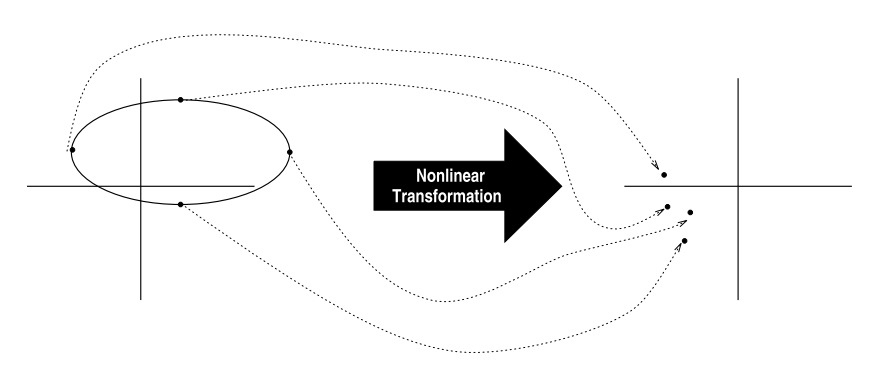
\includegraphics[width = 1\linewidth]{unscent.png}
    \caption[The principle of the Unscented Transform]{The principle of the Unscented Transform, where sigma points obtained by varying each dimension is the state space is propagated using the nonlinear model to approximate the distribution of the covariance, from \cite{julier1997new}}
    \label{fig:sec2_unscent}
\end{figure}

\begin{figure}[ht]
    \centering
    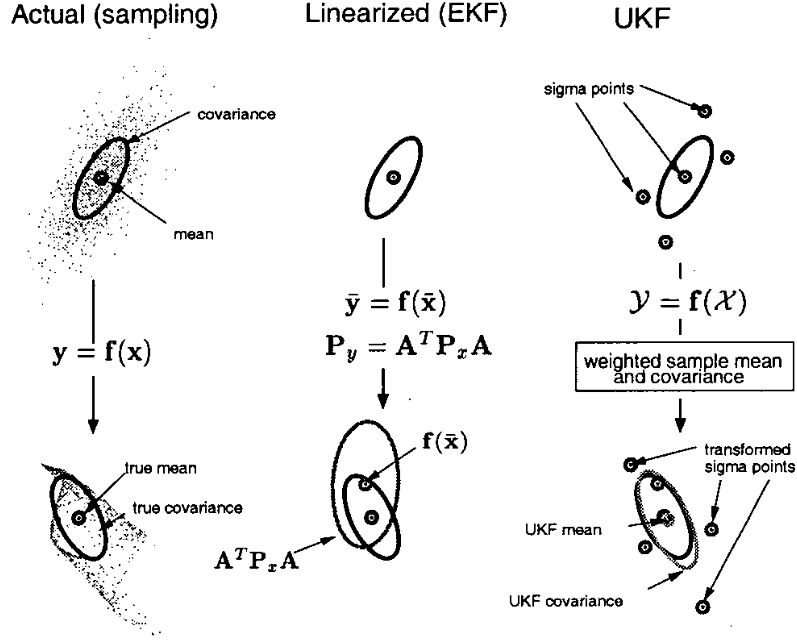
\includegraphics[width = 1\linewidth]{ekf_vs_ukf.png}
    \caption[Comparison of propagation between EKF and UKF]{Comparison of propagation between EKF and UKF. Left shows the true mean and covariance; middle represents the EKF approach, linearizing the system; right shows the UKF approach, generating sigma points (in this case, 5) to propagate the state and obtain estimation on the mean and covariance}
    \label{fig:w15_ekf_vs_ukf}
\end{figure}

These sigma points are given by Eqs.\,\eqref{eq:sec2_ukf_sigma1} to \eqref{eq:sec2_ukf_sigma3}, with corresponding weights $W_i$ associated to each point, where $L \in \mathbb{R}$ denotes the dimension of the state and $\kappa \in \mathbb{R}$ is a scaling parameter to control the spread of the sigma points. Furthermore, $\bar{x}$ represents the mean of state $x$, $P_{xx}$ its covariance, and $i \in [1,2n]$.

\begin{equation}
    \label{eq:sec2_ukf_sigma1}
    \chi_0 = \bar{x}, W_0 = \kappa /(L+\kappa)
\end{equation}
\begin{equation}
    \label{eq:sec2_ukf_sigma2}
    \chi_i = \bar{x} + \left( \sqrt{(L+\kappa)P_{xx}} \right), W_i = 1/2(L+\kappa)
\end{equation}
\begin{equation}
    \label{eq:sec2_ukf_sigma3}
    \chi_{i+L} = \bar{x} - \left( \sqrt{(L+\kappa)P_{xx}} \right), W_{i+L} = 1/2(L+\kappa)
\end{equation}

The propagation of the sigma points is then given by Eqs.\,\eqref{eq:sec2_ukf_sigma_exp1} to \eqref{eq:sec2_ukf_sigma_exp3}.

\begin{equation}
    \label{eq:sec2_ukf_sigma_exp1}
    y_i=f(\chi_i)
\end{equation}
\begin{equation}
    \label{eq:sec2_ukf_sigma_exp2}
    \bar{y} = \sum_{i=0}^{2L} W_i y_i
\end{equation}
\begin{equation}
    \label{eq:sec2_ukf_sigma_exp3}
    P_{yy} = \sum_{i=0}^{2L} \left( y_i - \bar{y} \right) \left( y_i - \bar{y} \right) ^T
\end{equation}

This transformation allows us to have the mean and covariance associated with the nonlinear process, without the need to linearize it beforehand, producing a better approximation as well. 

The full algorithm is given by Eqs.\,\eqref{eq:w15_ukf_first} through \eqref{eq:w15_ukf_last}.

\begin{myframe}[title=UKF algorithm, float]
    Initialize with:
    \begin{equation} \bar{x}_0=\mathbb{E}\left[ x_0 \right] \quad P_0=\mathbb{E}\left[ \left( x_0 - \bar{x}_0 \right) \left( x_0 - \bar{x}_0 \right)^T \right]\label{eq:w15_ukf_first} \end{equation}
    For $k \in \left\{ 1, \cdots, +\infty \right\}$

    Calculate sigma points:
    \begin{equation}
        \chi_{k-1} = \left[ \hat{x}_{k-1} \hat{x}_{k-1}+\eta \sqrt{P_{k-1}} \hat{x}_{k-1} \hat{x}_{k-1}-\eta \sqrt{P_{k-1}} \right]
    \end{equation}
    Time update:
    \begin{equation}
        \chi_{k|k-1}=F\left[ \chi_{k-1}, u_{k-1} \right]
    \end{equation}
    \begin{equation}
        \hat{x}_k^-=\sum_{i=0}^{2L}W_i\chi_{i,k|k-1}
    \end{equation}
    \begin{equation}
        P_k^-=\sum_{i=0}^{2L}W_i\left[ \chi_{i,k|k-1} - \hat{x}_k^- \right] \left[ \chi_{i,k|k-1} - \hat{x}_k^- \right]^T+R^v
    \end{equation}
    \begin{equation}
        y_{k|k-1} = H \left[ \chi_{k|k-1} \right]
    \end{equation}
    \begin{equation}
        \hat{y}_k^-=\sum_{i=0}^{2L}W_i y_{i,k|k-1}
    \end{equation}
    Measurement update equations:
    \begin{equation}
        P_{y_ky_k}=\sum_{i=0}^{2L}W_i \left[ y_{i,k|k-1} - \hat{y}_k^- \right] \left[ y_{i,k|k-1} - \hat{y}_k^- \right]^T +R^n
    \end{equation}
    \begin{equation}
        P_{x_ky_k}=\sum_{i=0}^{2L}W_i\left[ \chi_{i,k|k-1} - \hat{x}_k^- \right] \left[ y_{i,k|k-1} - \hat{y}_k^- \right]^T
    \end{equation}
    \begin{equation}
        \mathcal{K}_k=P_{x_ky_k}P_{x_ky_k}^{-1}
    \end{equation}\
    \begin{equation}
        \hat{x}_k=\hat{x}_k^- +\mathcal{K}_k \left( y_k - \hat{y}_k^- \right)
    \end{equation}
    \begin{equation} \label{eq:w15_ukf_last}
        P_k=P_k^--\mathcal{K}_kP_{y_ky_k}\mathcal{K}_K^T
    \end{equation}
    where $R^v$ is process noise covariance and $R^n$ is measurement noise covariance
\end{myframe}

%\begin{mymathbox}[ams gather, title=UKF algorithm, %colframe=blue!30!black]
%    \text{Initialize with:}\\
%    \bar{x}_0=\mathbb{E}\left[ x_0 \right]
%    \end{mymathbox}


%fdhsfjkhgks


%\begin{equation}
%    \label{eq:sec2_ukf_1}
%    \chi_i (k+1|k) = f (\chi_i(k|k),u(k))
%\end{equation}
%\begin{equation}
%%    \label{eq:sec2_ukf_2}
 %   \hat{x}(k+1|k) = \sum_{i=0}^{2n} W_i  \chi_i (k+1|k) 
%\end{equation}
%\begin{equation}
%    \label{eq:sec2_ukf_3}
%    P(k+1|k) = \sum_{i=0}^{2n} W_i \left[  \chi_i (k+1|k) - \hat{x}(k+1|k) \right]  \left[  \chi_i (k+1|k) - \hat{x}(k+1|k) \right]^T
%\end{equation}

%\begin{equation}
%    \label{eq:sec2_ukf_4}
%    Z_i(k+1|k) = h(\chi_i (k+1|k), u(k))
%\end{equation}
%\begin{equation}
%    \label{eq:sec2_ukf_5}
%    \hat{z}(k+1|k) = \sum_{i=0}^{2n} W_i Z_i(k+1|k)
%\end{equation}
%\begin{equation}
%    \label{eq:sec2_ukf_6}
%    P_{vv}(k+1|k) = R_1 + \sum_{i=0}^{2n} W_i \left[ Z_i(k|k-1) - \hat{z}(k+1|k) \right] \left[ Z_i(k|k-1) - \hat{z}(k+1|k) \right]^T
%\end{equation}
%\begin{equation}
%    \label{eq:sec2_ukf_7}
%    P_{xz} = \sum_{i=0}^{2n} W_i \left[ \chi_i(k|k-1) - \hat{x}(k+1|k) \right] \left[ Z_i(k|k-1) - \hat{z}(k+1|k) \right]^T
%\end{equation}

By using the UKF, it is not needed to linearize the system equations, which results in a better approximation of the uncertainty of the estimate, since the nonlinearities of the system are somewhat taken into account. Furthermore, the use of the unscented transform also makes the filter more robust to noise (\cite{wan2000unscented}).

\subsection{Square-Root Unscented Kalman Filter (SR-UKF)}
\label{sec:sec2_sr_ukf}

The most computationally expensive operation in the UKF is the generation of the new set of sigma points at each time update, that requires taking the matrix square root of the covariance matrix $P \in \mathbb{R}^{L\times L}$, which can be given by $P=SS^T$


\bibliographystyle{plain}
\bibliography{../thesis/ref}
% replace "project" by "thesis" if you are doing the thesis

\end{document}
